


\begin{frame}{Udsætning af gråænder}

\begin{columns}[T] % T = top-aligned

\begin{column}{0.48\textwidth}
\textbf{Regler i ferske vande:}
\begin{itemize}
    \item Kan udsættes 1. april til 31. juli
    \item 1 ælling pr. 150 m² åben vandflade
    \item Eller 1 voksen and pr. 300 m² åben vandflade
    \item Ingen generel ha-begrænsning som ved fasan/agerhøne
    \item Ingen biotopplan-krav for højere antal
    \item Alle udsætninger skal indberettes senest 1 uge efter udsætningen
    \item Over 100 fugle (samlet med fasan/agerhøne) kræver godkendt kursus
\end{itemize}
\end{column}

\begin{column}{0.3\textwidth}
    % Vælg én af disse – de ser godt ud i præsentation
    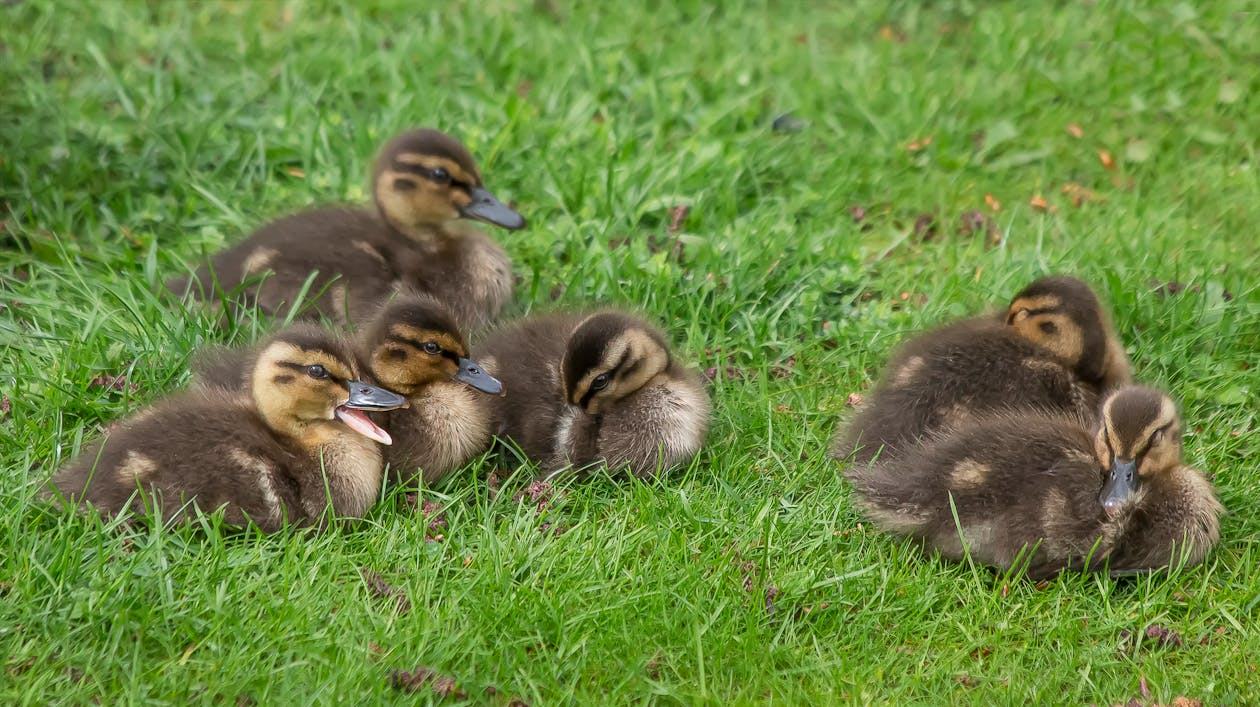
\includegraphics[width=\textwidth]{Billeder/Vildtforvaltning/udsætning/gråandeællinger.jpeg}
    % Eller brug et af de gode eksempler:
    % \includegraphics[width=\textwidth]{vegetationsstriber_midtmark_ex.jpg}
\end{column}

\end{columns}

\end{frame}